\bookchapter{How a Computer Works}\label{ch:hw1}

\section*{Explanation}
Your robot has a computer on its back, your laptop has one, and the servers that train neural networks have thousands. They differ in size, but they work in the same way. When a program is too slow, when the robot runs out of memory, or when a camera stream stutters, you need a picture of \emph{what is inside and how fast each part is}. This chapter gives you that picture, from the bit to the boot process, and it ties the numbers to the tools of Chapters~\ref{ch:linux8} and~\ref{ch:py8}.

\section*{Bits, bytes and numbers}
Everything in a computer is stored as \textbf{bits}, values $0$ or $1$. Eight bits make a \textbf{byte}, which can hold $2^8=256$ different values ($0\dots255$, exactly one pixel channel of an image, Chapter~\ref{ch:py10}). Humans write long bit patterns in \textbf{hexadecimal} (base $16$, digits \texttt{0--9a--f}): four bits are one hex digit.
\begin{verbatim}
>>> bin(202), hex(202), int("ca", 16), 0b1011
('0b11001010', '0xca', 202, 11)
>>> 2**8, 2**16, 2**32, 2**64
(256, 65536, 4294967296, 18446744073709551616)
\end{verbatim}
\begin{center}
\renewcommand{\arraystretch}{1.2}
\begin{tabular}{p{3.6cm}p{9.4cm}}
\textbf{Unit} & \textbf{Meaning}\\ \hline
$1$ kB, MB, GB, TB & $10^3,10^6,10^9,10^{12}$ bytes (manufacturers of disks and networks)\\
$1$ KiB, MiB, GiB & $2^{10}, 2^{20}, 2^{30}$ bytes (what \texttt{free -h} and \texttt{ls -lh} show)\\
Mbit/s & megabits per second, $=\tfrac18$ MB/s; network speeds are given in bits, files in bytes\\
\end{tabular}
\end{center}
\textbf{Whole numbers} are stored as binary numbers with a fixed number of bits ($8,16,32,64$); a \texttt{uint8} wraps around at $255$ (Chapter~\ref{ch:py8}). \textbf{Decimal numbers} use the floating-point format (IEEE~754), a binary scientific notation: a sign, an exponent and a mantissa (Figure~\ref{fig:hw1_float}).
\begin{center}
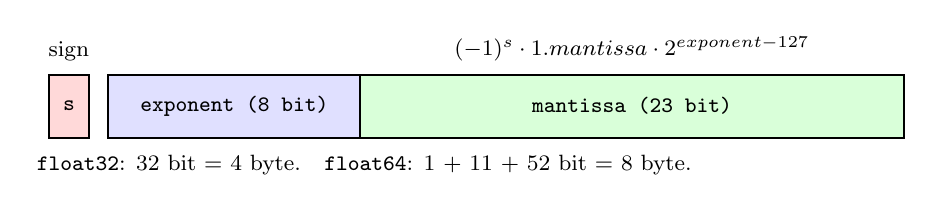
\begin{tikzpicture}[b/.style={draw,thick,minimum height=0.8cm,font=\footnotesize\ttfamily,inner sep=0pt}]
  \node[b,fill=red!15,minimum width=0.5cm] (s) at (0.25,0) {s};
  \node[b,fill=blue!12,minimum width=3.2cm] (e) at (2.35,0) {exponent (8 bit)};
  \node[b,fill=green!15,minimum width=6.9cm] (m) at (7.4,0) {mantissa (23 bit)};
  \node[font=\footnotesize,anchor=south] at (0.25,0.45) {sign};
  \node[font=\footnotesize,anchor=south] at (7.4,0.45) {$(-1)^s\cdot 1.\text{mantissa}\cdot 2^{\text{exponent}-127}$};
  \node[font=\footnotesize,anchor=north] at (4.0,-0.5) {\texttt{float32}: 32 bit = 4 byte.\quad \texttt{float64}: 1 + 11 + 52 bit = 8 byte.};
\end{tikzpicture}
\captionof{figure}{The layout of a \texttt{float32}. With $23$ mantissa bits it has about $7$ correct decimal digits; \texttt{float64} has about $16$.}\label{fig:hw1_float}
\end{center}
Consequences you have already met: $0.1$ has no exact binary form, so \texttt{0.1 + 0.2} is not $0.3$ (Chapter~\ref{ch:py1}); a \texttt{float32} cannot count above $2^{24}=16\,777\,216$ in steps of one (\texttt{np.float32(16777217)} gives \texttt{16777216.0}); the machine epsilon (the smallest relative step) is $1.2\cdot10^{-7}$ for \texttt{float32} and $2.2\cdot10^{-16}$ for \texttt{float64}. Neural networks run happily in \texttt{float32}, \texttt{float16} or even 8-bit integers: fewer bits mean less memory and faster calculation, at the price of precision.

\begin{example}
\textbf{How much data is a camera?} A colour image of $640\times480$ pixels with $3$ bytes per pixel is $640\cdot480\cdot3=921\,600$ bytes. At $30$ images per second that is $27.6$ MB/s, or $221$ Mbit/s. At $1920\times1080$ it is $186.6$ MB/s: more than a Wi-Fi link can carry, which is why cameras compress video (H.264/H.265 or MJPEG). \textbf{How much memory is a network?} A model with $25$ million parameters needs $25\cdot10^6\cdot4=100$ MB in \texttt{float32}, $50$ MB in \texttt{float16} and $25$ MB in 8-bit form.
\end{example}

\section*{The parts of a computer}
\begin{center}
\begin{tikzpicture}[b/.style={draw,rounded corners,thick,align=center,font=\footnotesize,minimum height=1.1cm},>={Stealth[length=2.5mm]}]
  \node[b,fill=blue!12,minimum width=3.4cm,minimum height=1.9cm] (cpu) at (0,0) {\textbf{CPU}\\cores, registers,\\caches};
  \node[b,fill=green!12,minimum width=3.0cm] (ram) at (5.0,0.8) {\textbf{RAM}\\working memory};
  \node[b,fill=orange!15,minimum width=3.0cm] (gpu) at (5.0,-0.9) {\textbf{GPU / NPU}\\parallel calculation};
  \node[b,fill=yellow!20,minimum width=3.4cm] (st) at (0,-3.0) {\textbf{storage}\\SSD / NVMe / SD};
  \node[b,fill=gray!15,minimum width=3.0cm] (io) at (5.0,-3.0) {\textbf{I/O}\\USB, Ethernet,\\Wi-Fi, CAN, GPIO};
  \draw[<->,thick] (cpu.east|-ram.west)--node[above,font=\scriptsize]{memory bus}(ram.west);
  \draw[<->,thick] (cpu.east|-gpu.west)--node[below,font=\scriptsize]{PCIe}(gpu.west);
  \draw[<->,thick] (cpu)--node[left,font=\scriptsize]{PCIe}(st);
  \draw[<->,thick] (cpu.south east)--(io.north west);
  \draw[<->,thick,dashed] (ram.south)--(gpu.north);
  \node[draw,dashed,rounded corners,gray,fit=(cpu)(ram)(gpu)(st)(io),inner sep=8pt] {};
  \node[font=\scriptsize,gray!60!black] at (2.5,-4.3) {on a laptop: separate chips on a board; on a robot computer: often one chip (SoC)};
\end{tikzpicture}
\captionof{figure}{The main parts of a computer and how they are connected.}\label{fig:hw1_blocks}
\end{center}
\begin{description}
  \item[CPU] (central processing unit) executes the instructions of programs, one after another, very fast, in a few \textbf{cores} that work independently. The \textbf{clock} ($2$ to $5$\,GHz, i.e.\ $2$ to $5\cdot10^9$ steps per second) paces the work; one step lasts a fraction of a nanosecond, and light travels only $10$\,cm in that time. A modern core finishes several instructions per step (the IPC of Chapter~\ref{ch:linux8}). Inside there are \textbf{registers} (a few dozen values, immediately usable) and \textbf{caches} (small, fast memory copies).
  \item[RAM] (random-access memory) holds the data and programs that are running. It is fast but \textbf{volatile}: its content disappears when the power goes. Typical: $8$ to $64$ GB on a laptop, $4$ to $16$ GB on a robot computer.
  \item[Storage] keeps data permanently: an \textbf{SSD} (flash memory chips, NVMe over PCIe is the fastest), an \textbf{SD card} or eMMC on small boards; hard disks with spinning platters are slow and fragile, so they do not belong in a moving robot.
  \item[GPU] (graphics processing unit): thousands of small cores that do the \emph{same} operation on much data at once. Neural networks consist of huge matrix multiplications (Chapter~\ref{ch:py8}), exactly this kind of work, so a GPU is $10$ to $100$ times faster than a CPU for them. An \textbf{NPU} is a chip specialised for neural network inference (the ``TOPS'' figure in the data sheet means trillions of operations per second, usually 8-bit).
  \item[I/O] connects the world: USB cameras, Ethernet and Wi-Fi, serial ports and \textbf{GPIO} pins, and buses such as I2C, SPI and CAN (Chapter~\ref{ch:hw3}).
\end{description}
\textbf{x86 and ARM.} Laptops and servers mostly have \textbf{x86-64} processors (Intel, AMD). Phones, single-board computers (Raspberry Pi) and many robots use \textbf{ARM} (\texttt{aarch64}), which is more efficient per watt. A program compiled for one does not run on the other, packages must match (\verb!uname -m! tells you which you have, Chapter~\ref{ch:linux4}). Python code runs on both; compiled libraries come in two builds. A \textbf{SoC} (system on a chip) puts CPU, GPU, memory controller and I/O on one chip; robot computers such as the NVIDIA Jetson boards are SoCs with an integrated GPU that shares the RAM with the CPU.

\subsection*{Looking at your own machine}
\begin{verbatim}
$ lscpu | head -4                  # CPU model, cores, clock, caches
$ nproc                            # number of cores
$ free -h                          # RAM (Chapter 8)
$ lsblk                            # disks and partitions
$ lspci ; lsusb                    # devices on the PCIe and USB buses
$ nvidia-smi                       # NVIDIA GPU: load, memory, temperature
$ sudo dmesg | tail         # what the kernel noticed (devices, errors)
$ uname -m                         # x86_64 or aarch64
\end{verbatim}
On a typical cloud machine \texttt{lscpu} reports, for example, \texttt{Model name: Intel(R) Xeon(R) Processor @ 2.10GHz} with $2$ cores and \texttt{free -h} shows $7.8$ GiB total memory. Learn to read these once; every bug report from a robot should start with them (Chapter~\ref{ch:linux8}).

\section*{The memory hierarchy}
The central fact of computer performance: a fast memory is small and expensive, a large memory is slow. So computers stack several levels, each a cache for the next (Figure~\ref{fig:hw1_hier}).
\begin{center}
\begin{tikzpicture}[>={Stealth[length=2.5mm]}]
  \foreach \i/\w/\n/\sz/\lat/\col in {0/1.6/registers/{$<$ 1 kB}/{0.3 ns}/red!25, 1/3.0/{L1 cache}/{32--64 kB}/{1 ns}/orange!30, 2/4.4/{L2 cache}/{0.5--2 MB}/{4 ns}/yellow!35, 3/5.8/{L3 cache}/{8--64 MB}/{15 ns}/green!25, 4/7.2/{RAM}/{8--64 GB}/{80 ns}/cyan!20, 5/8.6/{SSD (NVMe)}/{256 GB--4 TB}/{80 $\mu$s}/blue!15}{
    \node[draw,thick,fill=\col,minimum width=\w cm,minimum height=0.8cm,font=\footnotesize] at (0,-0.85*\i) {\n};
    \node[font=\footnotesize,anchor=west] at (4.6,-0.85*\i) {\sz};
    \node[font=\footnotesize\bfseries,anchor=west,blue!50!black] at (7.5,-0.85*\i) {\lat};
  }
  \node[font=\footnotesize,anchor=west] at (4.6,0.6) {size};
  \node[font=\footnotesize,anchor=west] at (7.5,0.6) {typical delay};
  \draw[->,thick] (-4.8,0.2)--(-4.8,-4.4) node[midway,left,rotate=90,anchor=south,font=\footnotesize]{slower, larger};
\end{tikzpicture}
\captionof{figure}{The memory hierarchy with typical orders of magnitude (exact values depend on the chip). A program that has to wait for RAM waits for about $80$ ns, i.e.\ roughly $250$ clock steps; a network packet takes $10^6$ times longer than a register access.}\label{fig:hw1_hier}
\end{center}
Memory is moved in blocks of $64$ bytes (a \textbf{cache line}). If your program reads neighbouring values one after another, the first read loads the line and the next ones are free. If it jumps around, every access waits for RAM. This is the reason for the $3$-fold difference between walking through a table by rows and by columns that you measured in Chapter~\ref{ch:linux8}, and one more reason why NumPy arrays (contiguous memory) are much faster than Python lists of objects (Chapter~\ref{ch:py8}). Rules of thumb:
\begin{itemize}[nosep]
  \item Work on data in the order in which it lies in memory.
  \item Keep the working set small; a model that fits into the cache runs faster.
  \item Disk and network are \emph{thousands to millions} of times slower than RAM: never read a file or call a network service inside a fast loop; load once and keep it in memory.
  \item When RAM is full, Linux uses swap on the disk and the program slows down dramatically, or the OOM killer ends a process (Chapter~\ref{ch:linux8}).
\end{itemize}

\section*{What happens when you press the power button}
\begin{center}
\begin{tikzpicture}[b/.style={draw,rounded corners,thick,minimum width=2.2cm,minimum height=1.0cm,align=center,font=\footnotesize},>={Stealth[length=2.5mm]}]
  \node[b,fill=gray!15] (a) at (0,0) {firmware\\UEFI / boot ROM};
  \node[b,fill=blue!10] (b) at (3.0,0) {bootloader\\GRUB};
  \node[b,fill=blue!15] (c) at (6.0,0) {kernel\\Linux};
  \node[b,fill=green!12] (d) at (9.0,0) {init\\systemd};
  \node[b,fill=orange!15] (e) at (12.0,0) {services,\\login, your program};
  \foreach \x/\y in {a/b,b/c,c/d,d/e}{\draw[->,thick] (\x)--(\y);}
\end{tikzpicture}
\captionof{figure}{The boot chain. Each stage loads and starts the next.}\label{fig:hw1_boot}
\end{center}
The \textbf{firmware} on a chip on the board tests the hardware and finds a bootable disk. The \textbf{bootloader} loads the \textbf{kernel} into RAM. The kernel starts the drivers, mounts the file system and starts the first process, \texttt{systemd} (process number $1$, Chapter~\ref{ch:linux5}), which starts the services and finally your robot program, if you configured a service for it. When a robot does not boot, you can usually tell in which stage it failed: no screen output (firmware or power), a boot menu error (bootloader or disk), a kernel message list (\texttt{dmesg}) that stops (driver or file system), or services that fail (\texttt{systemctl --failed}, \texttt{journalctl -b}). \texttt{journalctl -b -1} shows the log of the \emph{previous} boot, useful after a crash.

A \textbf{kernel} is the part of the operating system that controls the hardware and gives each program the illusion that it has the whole machine: it divides CPU time between processes, manages memory and offers files and network sockets through \textbf{system calls}. Programs never touch the hardware directly, drivers in the kernel do (Chapter~\ref{ch:linux6}).

\begin{keyidea}[Speed is a question of where the data is]
When something is slow, ask: is it waiting for the \textbf{CPU} (calculation, one core at 100\,\%), for \textbf{memory} (cache misses, swapping), for the \textbf{disk}, for the \textbf{network}, or for the \textbf{GPU}? The tools of Chapter~\ref{ch:linux8} answer this; this chapter gave you the numbers to judge the answer.
\end{keyidea}

\section*{Practice problems}
\begin{enumerate}[label=\textbf{\thechapter.\arabic*}]
  \item Convert $202$ to binary and hexadecimal by hand, and \texttt{0xff} and \texttt{0b101101} to decimal. Check in Python.
  \item How many different values can $n$ bits store? How many bits do you need for $1000$ different values?
  \item A $1280\times720$ gray image (one byte per pixel) at $60$ fps: how many MB/s? And in Mbit/s? Can it travel over a $100$ Mbit/s Ethernet link without compression?
  \item A network has $60$ million parameters. How many MB does it need in \texttt{float32}, \texttt{float16} and \texttt{int8}? Does it fit into a $32$ MB L3 cache in each case?
  \item Why does \texttt{0.1 + 0.2 != 0.3}? How many decimal digits can a \texttt{float32} hold reliably?
  \item List the levels of the memory hierarchy and explain why computers do not simply use the fastest kind everywhere.
  \item Why is a Python loop over a NumPy array slower than the vectorised operation, from the point of view of the hardware (name two reasons)?
  \item What is the difference between RAM and an SSD, and what happens to each when the power fails?
  \item Why is a GPU good for neural networks and a CPU better for a program with many \texttt{if} decisions?
  \item[\textbf{\thechapter.10}$\star$] A robot computer will not start. The screen stays black, no network. Describe a systematic plan to find out in which stage of the boot chain it fails, naming the tools you use at each stage.
\end{enumerate}
